% TikZ system overview diagram for RoboPhD
% Shows: Simple Inputs → Evolutionary Process → Strong Output

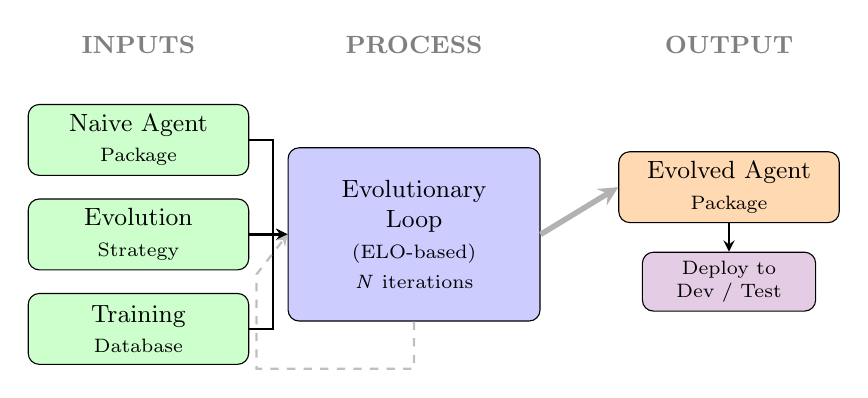
\begin{tikzpicture}[
    % Node styles
    input/.style={draw, rounded corners, fill=green!20, minimum width=2.8cm, minimum height=0.9cm, align=center, font=\small},
    process/.style={draw, rounded corners, fill=blue!20, minimum width=3.2cm, minimum height=2.2cm, align=center, font=\small},
    output/.style={draw, rounded corners, fill=orange!30, minimum width=2.8cm, minimum height=0.9cm, align=center, font=\small},
    deploy/.style={draw, rounded corners, fill=violet!20, minimum width=2.2cm, minimum height=0.7cm, align=center, font=\scriptsize},
    arrow/.style={->, >=stealth, thick},
    bigarrow/.style={->, >=stealth, line width=2pt, color=gray!60},
    label/.style={font=\scriptsize, color=gray!70}
]

% Section labels
\node[font=\small\bfseries, color=gray] at (-3.5, 2.2) {INPUTS};
\node[font=\small\bfseries, color=gray] at (0, 2.2) {PROCESS};
\node[font=\small\bfseries, color=gray] at (4, 2.2) {OUTPUT};

% Input nodes (left)
\node[input] (naive) at (-3.5, 1) {Naive Agent\\{\scriptsize Package}};
\node[input] (strategy) at (-3.5, -0.2) {Evolution\\{\scriptsize Strategy}};
\node[input] (training) at (-3.5, -1.4) {Training\\{\scriptsize Database}};

% Process node (center)
\node[process] (evolution) at (0, -0.2) {Evolutionary\\Loop\\{\scriptsize (ELO-based)}\\{\scriptsize \textit{N} iterations}};

% Output node (right)
\node[output] (evolved) at (4, 0.4) {Evolved Agent\\{\scriptsize Package}};
\node[deploy] (deploy) at (4, -0.8) {Deploy to\\Dev / Test};

% Arrows from inputs to process
\draw[arrow] (naive.east) -- ++(0.3,0) |- (evolution.west);
\draw[arrow] (strategy.east) -- (evolution.west);
\draw[arrow] (training.east) -- ++(0.3,0) |- (evolution.west);

% Big arrow from process to output
\draw[bigarrow] (evolution.east) -- (evolved.west);

% Arrow from output to deploy
\draw[arrow] (evolved.south) -- (deploy.north);

% Dotted feedback loop (optional - shows iteration)
\draw[arrow, dashed, color=gray!50] (evolution.south) -- ++(0, -0.6) -- ++(-2, 0) -- ++(0, 1.2) -- (evolution.west);

\end{tikzpicture}
